\exkw{Fachwerk}
\exkw{Balken}
\exkw{Moment}
\exkw{Kraft}
\exquestion{Ebenes Fachwerk}

Gegeben sei folgendes ebenes Fachwerk:

\begin{center}
	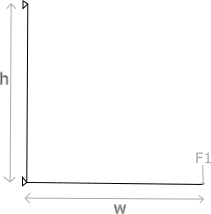
\includegraphics[width=0.5\columnwidth]{./FachwerkEben_1.png}
\end{center}

Berechne:

\begin{itemize}
	\item Allgemein die auftretenden Auflagerkräfte im oberen und unteren Lager,
		wenn das Eigengewicht des Trägers ignoriert wird.
	\item Allgemein alle auftretenden Schnittkräfte, wenn das Eigengewicht des
		Trägers ignoriert wird.
	\item Die auftretenden Auflagerkräfte sowie Schnittkräfte, wenn das Eigengewicht
		des Trägers durch die differentielle Kraft $q$ gegeben ist.
	\item Berechne die auftretenden Kräfte, wenn die Eigenlast durch die Differentielle
		Kraft $q=6,9 \frac{\text{kg}}{\text{m}}$, die Höhe $h=20\text{cm}$, die Länge
		ebenfalls $w=20\text{cm}$ beträgt und die Kraft $F_1$ durch ein $1.7\text{kg}$
		schweres Objekt bei einer Erdbeschleunigung von ca. $g\approx10 \frac{\text{m}}{\text{s^2}}$
		hervorgerufen wird.
\end{itemzie}